 \documentclass[a4paper, 10pt, final]{article}

\usepackage{a4wide}

\usepackage{charter}
\usepackage{verbatim}
\usepackage{amsfonts}
\usepackage{amsmath}
\usepackage{amsthm}
\usepackage{amssymb}
%\usepackage[integrals]{wasysym}
%\usepackage{mathrsfs}
%\usepackage[mathcal]{euscript}
\usepackage{listings}
\usepackage{graphicx}
\usepackage{multirow}
\usepackage{hyperref}
\usepackage{float}
\usepackage[small,bf]{caption}
%\usepackage{xypic}
\usepackage[table]{xcolor}
\usepackage{subfig}
%\usepackage{ulem} %use \normalem after begin document
\usepackage[authoryear]{natbib}

% Settings
\parindent=5pt
\parskip=8pt plus 2pt minus 4pt
\lstset{language=Matlab, basicstyle=\scriptsize,
    showstringspaces=false, numbers=left, stepnumber=1, numberstyle=\tiny, frame=tb}


%% \def\mytitle{Signal and Image Processing 2010}
%% \def\mysubtitle{Handin of mandatory excercise 1}
%% \def\myauthor{Ulrik Bonde}
%% \def\mymail{\mailto{bonde@diku.dk}}
%% \def\mydate{\today}

\title{Statistical Methods for Machine Learning \\ Mandatory Project 1}
\author{Kasper Steenstrup\\Michael Andersen\\Esben Skaarup}
\date{\today}

%% \title{\mytitle}
%% \subtitle{\mysubtitle}

%% \author{\myauthor{} - \mymail}
%% \date{\mydate}

\hypersetup{
colorlinks,%
citecolor=black,%
filecolor=black,%
linkcolor=black,%
urlcolor=black,%
bookmarksopen=false,
pdftitle={Statistical Methods for Machine Learning - Mandatory Project 1},
pdfauthor={Kasper Steenstrup, Michael Andersen \& Esben Skaarup}
}

\begin{document}
\maketitle

\subsection*{Question 1.1 and 1.2}

In figure \ref{fig:q1_1} can be seen the $100$ data points drawn from
the gaussian distribution with $\mu = [1.0~ 1.0]$ and $\Sigma = [0.3~
  0.2; 0.2~ 0.2]$. The correct $\mu$ is blue and $\widehat{\mu}$ is
marked with red.

\begin{figure}[!htpb]
  \centering
  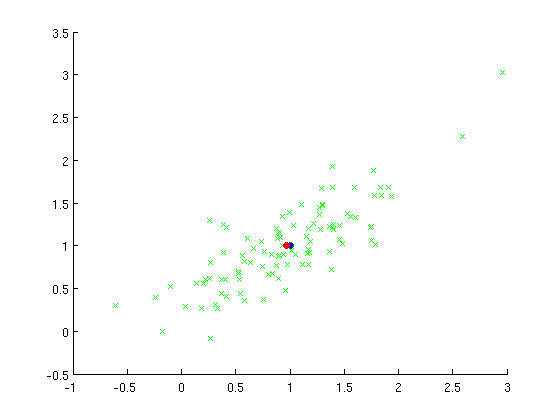
\includegraphics[width=0.6\textwidth]{images/q1_1}
  \caption{100 data points, correct mean with blue and estimated mean red.}
  \label{fig:q1_1}
\end{figure}

To quantify how much the estimated mean deviates from the correct
mean, we use usual euclidean distance between the two vectors.

Our distance is $0.0392$, which is not very much. This can also be
seen from the drawing, the points are placed really close.

\subsection*{Question 1.3}

\begin{figure}[!htpbpb]
  \centering
  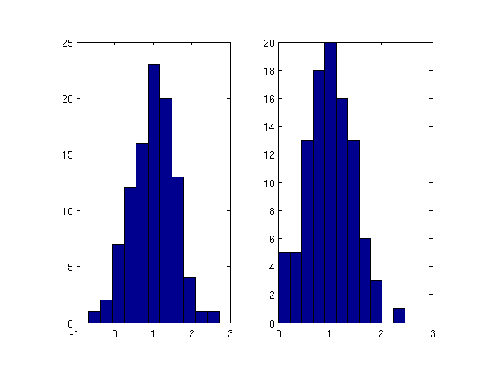
\includegraphics[width=0.6\textwidth]{images/q1_3a}
  \caption{a shows $p(x_1)$ and b shows $p(x_2)$ using 11 bins.}
  \label{fig:q3_3a}
\end{figure}

\begin{figure}[!htpb]
  \centering
  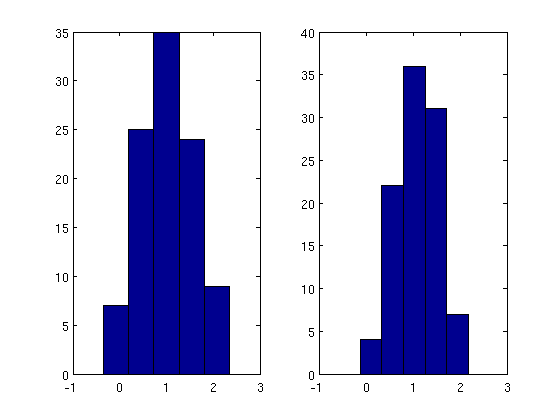
\includegraphics[width=0.6\textwidth]{images/q1_3b}
  \caption{a shows $p(x_1)$ and b shows $p(x_2)$ using 5 bins.}
  \label{fig:q3_3b}
\end{figure}

\begin{figure}[!htpb]
  \centering
  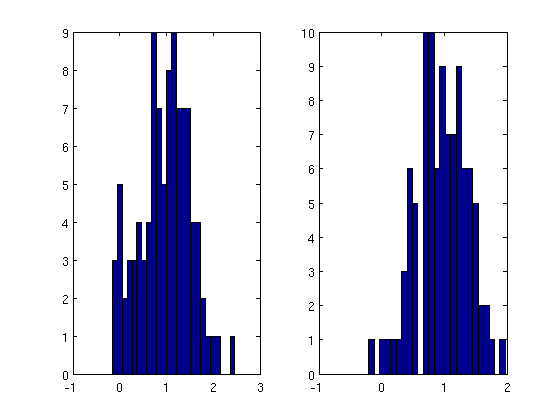
\includegraphics[width=0.6\textwidth]{images/q1_3c}
  \caption{a shows $p(x_1)$ and b shows $p(x_2)$ using 25 bins.}
  \label{fig:q3_3c}
\end{figure}

There is no best way to select the bin width. If it is selected too
small, the resulting density becomes very spiky and unable to capture
the structure of the distribution. Selecting the bin width too large,
can result in bimodal structure of the distribution being lost. So one
needs to use some intermediate value as bin width. In our case,
selecting a total of 11 bins seems to provide a good estimation of the
distribution, as seen in figure \ref{fig:q1_3a}, \ref{fig:q1_3b}, and \ref{fig:q1_3c}.

\subsection*{Question 1.4}

From the figures \ref{fig:q1_4_100}-\ref{fig:q1_4_10000_b20} it can be seen that
the gaussian distribution is rotated because the $\Sigma$-matrix different
values in the diagonal. The figures show the same tendency as in question 1.3
and can be solved by looking at the figures and selecting appropriate bin
numbers.

\begin{figure}[!htpb]
  \centering
  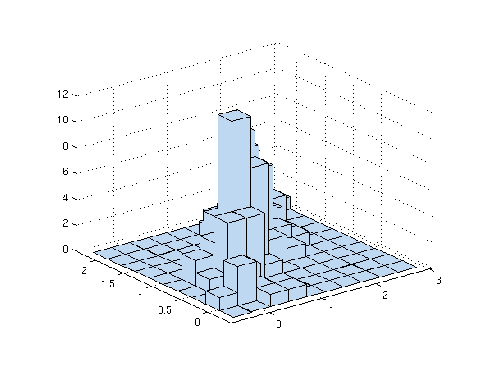
\includegraphics[width=0.6\textwidth]{images/q1_4_100}
  \caption{Shows 3d histogram of 100 datapoints using $10$x$10$ bins}
  \label{fig:q4_4_100}
\end{figure}

\begin{figure}[!htpb]
  \centering
  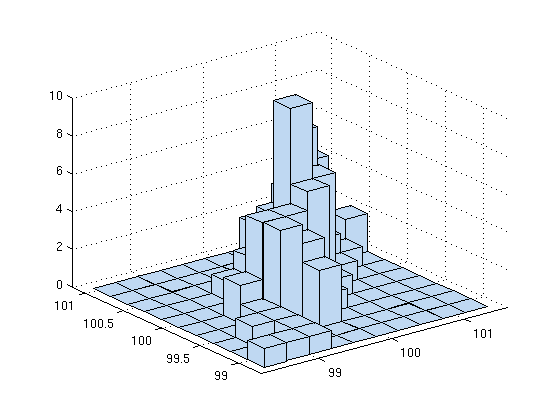
\includegraphics[width=0.6\textwidth]{images/q1_4_1000}
  \caption{Shows 3d histogram of 1000 datapoints using $10$x$10$ bins}
  \label{fig:q4_4_1000}
\end{figure}

\begin{figure}[!htpb]
  \centering
  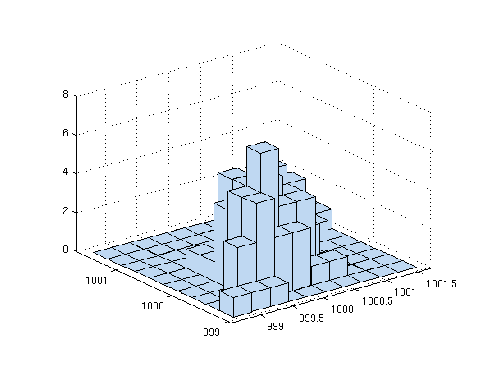
\includegraphics[width=0.6\textwidth]{images/q1_4_10000}
  \caption{Shows 3d histogram of 10000 datapoints using $10$x$10$ bins}
  \label{fig:q4_4_10000}
\end{figure}

\begin{figure}[!htpb]
  \centering
  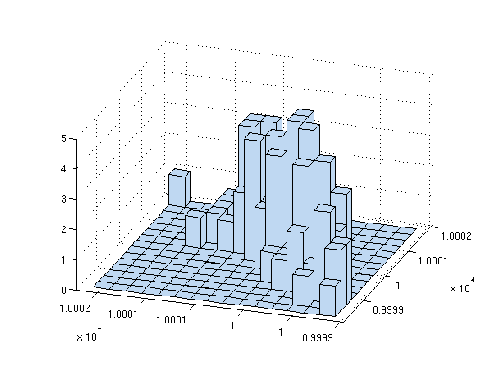
\includegraphics[width=0.6\textwidth]{images/q1_4_10000_b15}
  \caption{Shows 3d histogram of 10000 datapoints using $15$x$15$ bins}
  \label{fig:q4_4_10000_b15}
\end{figure}

\begin{figure}[!htpb]
  \centering
  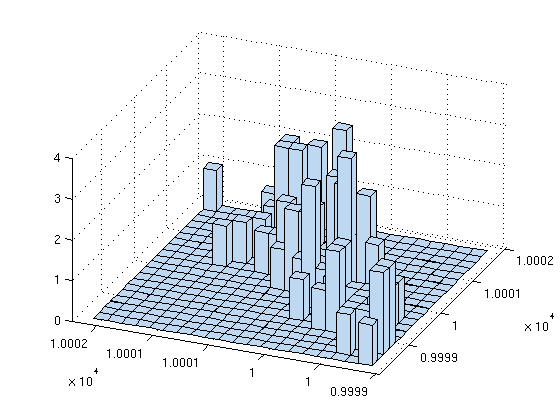
\includegraphics[width=0.6\textwidth]{images/q1_4_10000_b20}
  \caption{Shows 3d histogram of 10000 datapoints using $20$x$20$ bins}
  \label{fig:q4_4_10000_b20}
\end{figure}

\subsection*{Question 1.5}
In graph \ref{fig:q5} shows the difference between $\mu _y$, $\hat{y}$ convergence to 0 as $L -> \infty$

\begin{figure}[!ht]
  \centering
  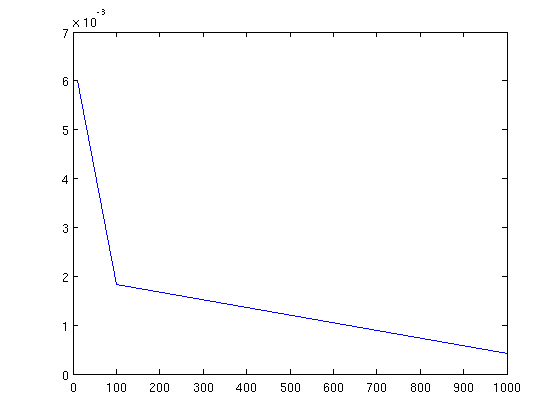
\includegraphics[width=0.6\textwidth]{images/q5_L10_L100_L1000}
  \caption{Shows the difference between $\mu _y$ and $\hat{y}$, at point 10, 100, 1000}
  \label{fig:q5}
\end{figure}

In graph \ref{fig:q5_log} we have taken the log of the difference, and
since the difference is an approximation for an exponential function, the
plotted line should be linear. It isn't quite linear, though, because of the bad
approximation and the large step size.

\begin{figure}[!ht]
  \centering
  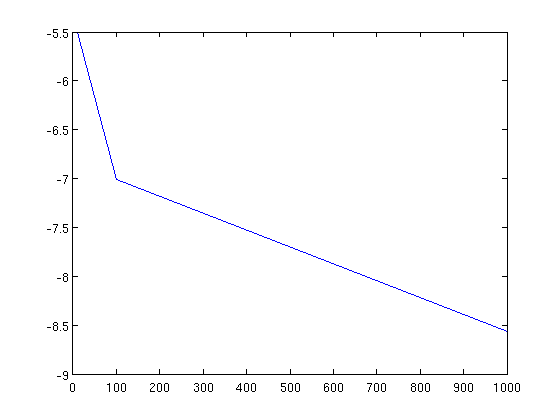
\includegraphics[width=0.6\textwidth]{images/q5_L10_L100_L1000_log}
  \caption{Shows the logarithm difference between $\mu _y$ and $\hat{y}$, at point 10, 100, 1000}
  \label{fig:q5_log}
\end{figure}

\subsection*{Question 1.6}

The auto-correlation is non-zero since we have few samples, and they
are distributes randomly. If we increase the number of samples $L$, the
auto-correlation gets smaller, see figure \ref{L10000}. When running the
program many times, we get different results, but the pattern is the same.
If we set $L$ to $10000$, the auto-correlation gets very small and changes
less between runs, see figure \ref{L10000}. This is as we expected, since
more samples, decreases the distance between the points.

\begin{figure}[!htpb]
  \centering
  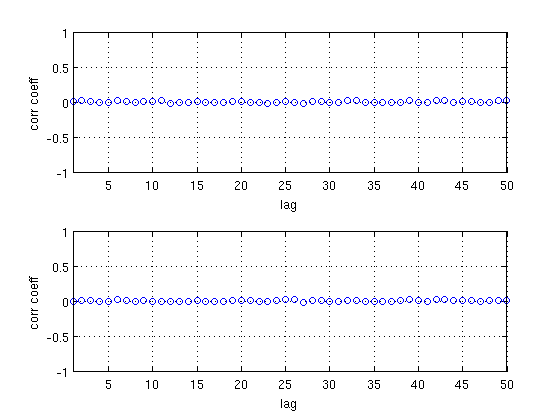
\includegraphics[width=0.6\textwidth]{images/L10000}
  \caption{auto-correlation, when $L = 10000$}
  \label{L10000}
\end{figure}
\newpage
\newpage
\newpage
\newpage
\newpage

%% \begin{figure}
%% \centering
%% \subfloat[]{\includegraphics[width=0.3\textwidth]{images/img00}}
%% \subfloat[]{\includegraphics[width=0.45\textwidth]{images/img00h}}
%% \caption{Original image and histogram, unadjusted}
%% \label{fig:original}
%% \end{figure}

\subsection*{Question 1.7}

\begin{figure}[!htpb]
  \centering
  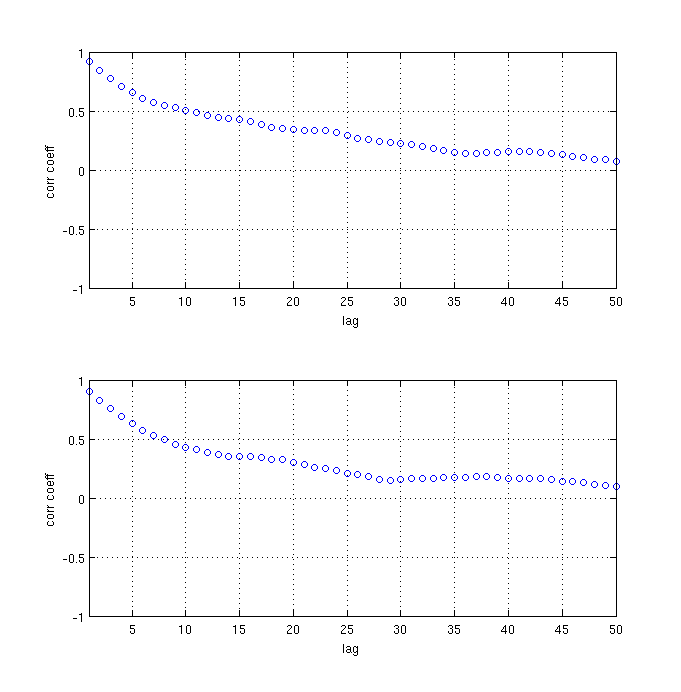
\includegraphics[width=0.6\textwidth]{images/q1_7a}
  \caption{Shows the autocorrelation plot of Metropolis-Hastings algorithm, running 500 samples, using 0.5 stepsize.}
  \label{fig:q1_7a}
\end{figure}

From figure \ref{fig:q1_7a} is can be seen that at first the samples
are dependant on each other but as the random walk progresses they
become more and more independent. And when reaching lag $50$ they are
nearly independent. From figure \ref{fig:q1_7b} the result of the
accepted samples from the random walk can be seen.

\begin{figure}[!htpb]
  \centering
  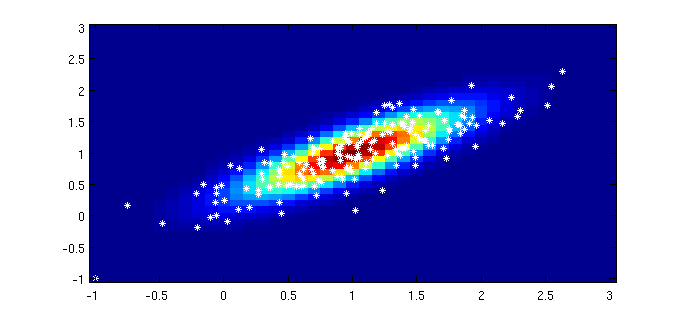
\includegraphics[width=0.6\textwidth]{images/q1_7b}
  \caption{}
  \label{fig:q1_7b}
\end{figure}

Give a rough estimate of the number of rejected samples

The proposal distribution is a gaussian distribution as a result of
using \emph{randn} in matlab. If the proposal distribution appeared in
the acceptance distribution, it would mean that the proposal
distribution itself was not simple and fast to calculate. 

Figure \ref{fig:q1_7c} show the autocorrelation using stepsize $0.2$,
because we do not take that long steps, we need more samples to obtain
independance between them. It also shows that within lag $50$ we do
not get that close to $0$. Figure \ref{fig:1_7d} show the resulting
distribution and accepted samples.

\begin{figure}[!htpb]
  \centering
  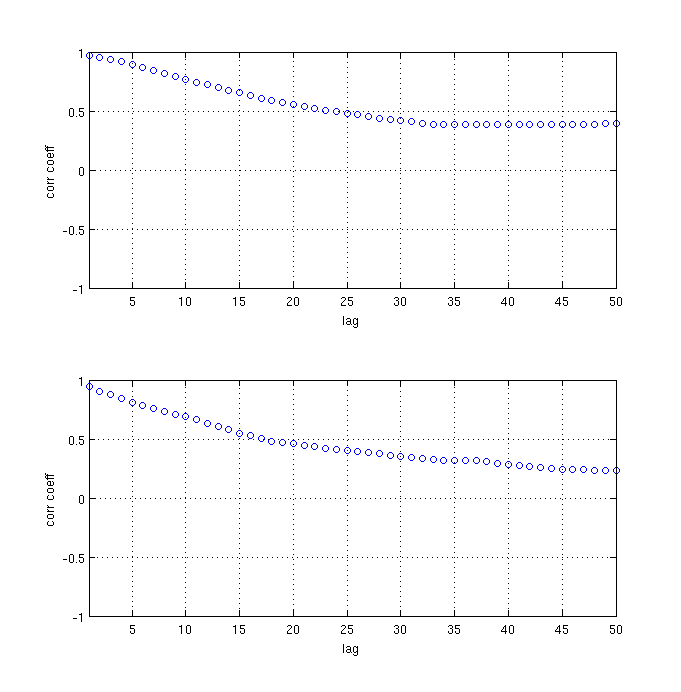
\includegraphics[width=0.6\textwidth]{images/q1_7c}
  \caption{}
  \label{fig:q1_7c}
\end{figure}

\begin{figure}[!htpb]
  \centering
  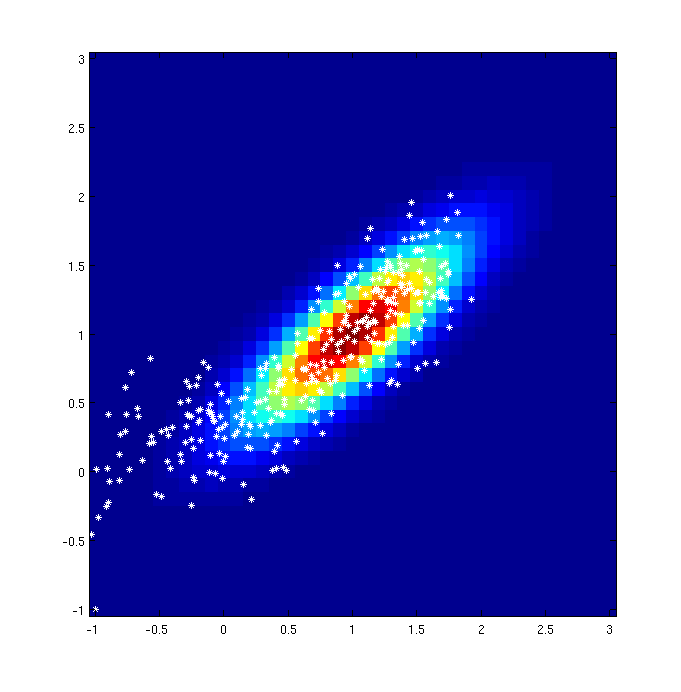
\includegraphics[width=0.6\textwidth]{images/q1_7d}
  \caption{}
  \label{fig:q1_7d}
\end{figure}

Changing the stepsize to $0.9$ seems to be an appropiate choice, the autocorrelation now converges fast towards zero. Although we are now forced to take large steps. This can be seen by looking at the figure \ref{fig:q1_7e}-\ref{fig:q1_7f}


\begin{figure}[!htpb]
  \centering
  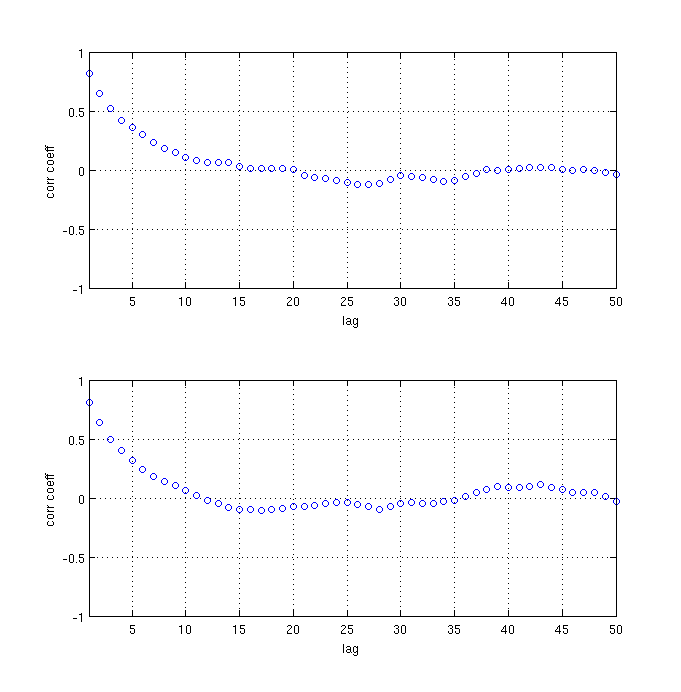
\includegraphics[width=0.6\textwidth]{images/q1_7e}
  \caption{}
  \label{fig:q1_7e}
\end{figure}

\begin{figure}[!htpb]
  \centering
  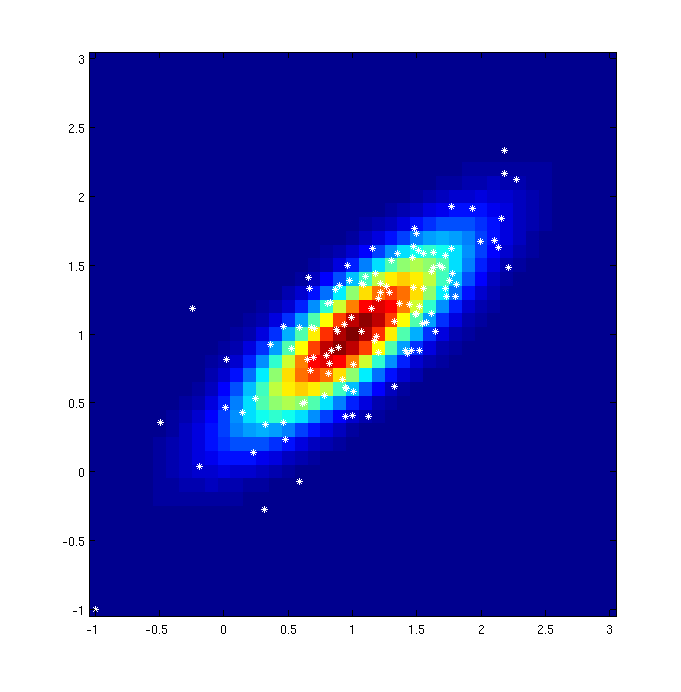
\includegraphics[width=0.6\textwidth]{images/q1_7f}
  \caption{}
  \label{fig:q1_7f}
\end{figure}

Using a larger stepsize results in the random walk stepping outside of the distribution, as we step outside of many times, a larger proportion of samples will be accepted.
An optimal value would be problem dependent, and would not apply to if transferred to another problem, but our best choice would be $0.9$ as it seems to converge fastest.

\begin{figure}[!htpb]
  \centering
  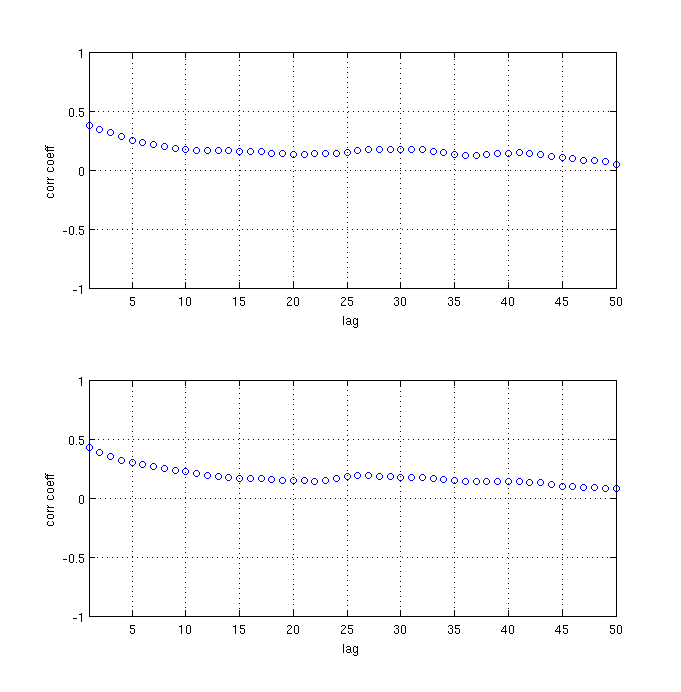
\includegraphics[width=0.6\textwidth]{images/q1_7g}
  \caption{}
  \label{fig:q1_7g}
\end{figure}

\begin{figure}[!htpb]
  \centering
  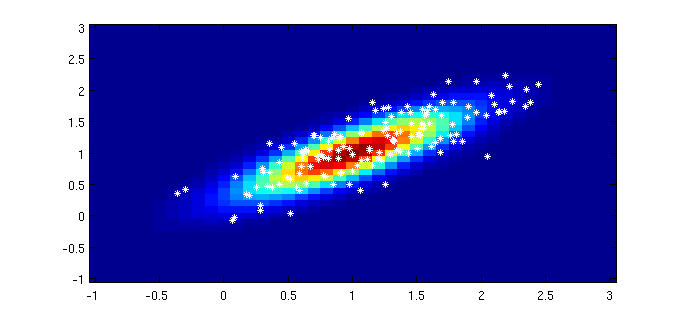
\includegraphics[width=0.6\textwidth]{images/q1_7h}
  \caption{}
  \label{fig:q1_7h}
\end{figure}

The two figures \ref{fig:q1_7g} and \ref{fig:q1_7h} shows when we discard the first $250$ samples, this results in most of the remaining samples being accepted. Though we could probably go even further and discard even more, especially if we chose more samples instead of $500$.


\begin{figure}[!htpb]
  \centering
  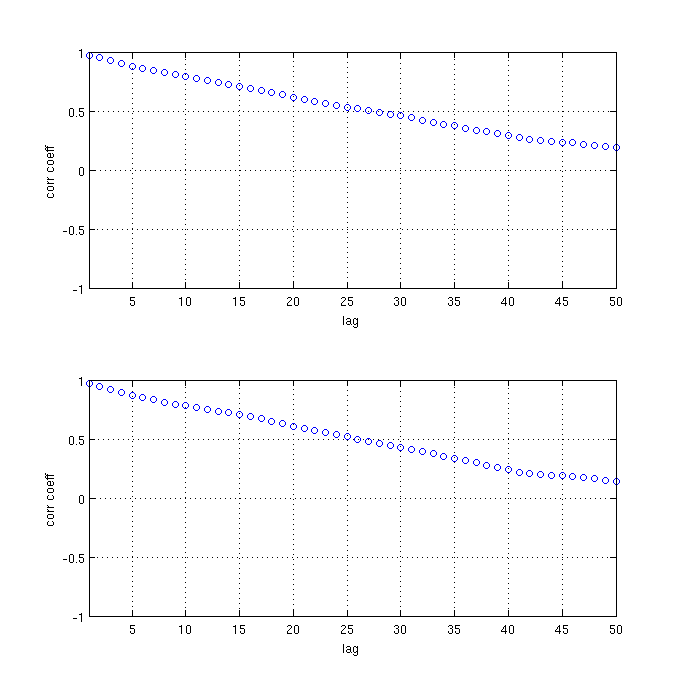
\includegraphics[width=0.6\textwidth]{images/q1_7i}
  \caption{}
  \label{fig:q1_7i}
\end{figure}

\begin{figure}[!htpb]
  \centering
  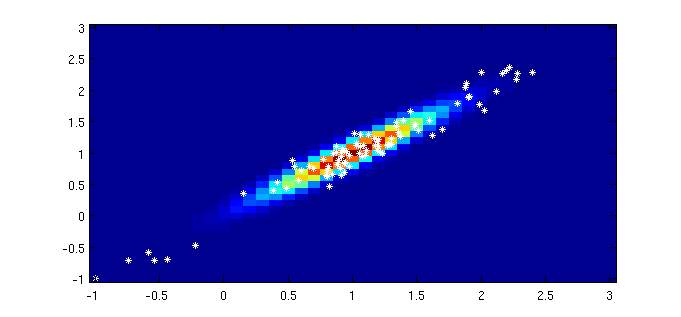
\includegraphics[width=0.6\textwidth]{images/q1_7j}
  \caption{}
  \label{fig:q1_7j}
\end{figure}

The figures \ref{fig:q1_7i} and \ref{fig:q1_7j} shows what happens when $|\Sigma|$ is nearly singular, this causes the longer burn-in. The autocorrelation converges slower towards zero. The effective number of samples will be problem dependent, because it will dependent on the acceptance distribution. If the acceptance distribution is close to singular, this means slower autocorrelation and the need to sample more in order to get effective samples.

\subsection*{Question 1.8}

The maximum likelihood estimation of the color yields the value $\mu _{ML} = [0.9556~ 0.2994~ 0.2569]$.
This seems reasonable for the red vase, as the red value is much larger than the green and blue ones.
Visualizing the RGB color gives a color very close to the color of the vase.

The covariance matrix is also calculated on the training data:\\
$$\Sigma _{ML} = \left[
\begin {array}{ccc}
0.0082 & 0.0052 & 0.0067\\
\noalign{\medskip}
0.0052 & 0.0171 & 0.0199\\
\noalign{\medskip}
0.0067 & 0.0199 & 0.0241\\
\end {array}
\right]$$
% [0.0082~ 0.0052~ 0.0067; 0.0052~ 0.0171~ 0.0199; 0.0067~ 0.0199~ 0.0241]

The probability for each pixel is visualized in figure \ref{fig:q1_8}.
The shape of the vase is clearly depicted, and no pixels outside the vase are visibly colored.
The lighter colors of the vase are not as accurately identified, especially where the reflections cause the original image to have white parts.
This is expected, as the light colors are underrepresented in the training data, causing the $\mu _{ML}$ to be far from white.

\begin{figure}[!htpb]
  \centering
  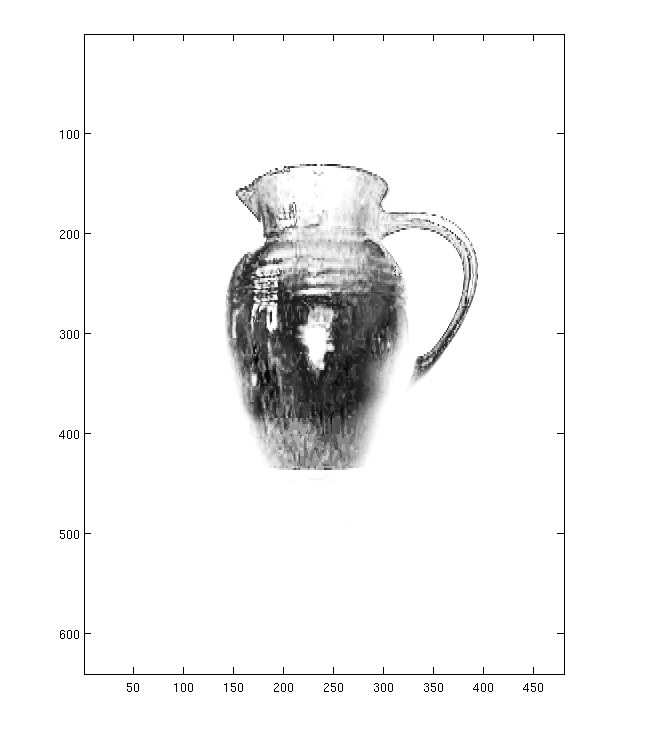
\includegraphics[width=0.6\textwidth]{images/kande1_probebility.png}
  \caption{The probability of each pixel being a part of the vase.}
  \label{fig:q1_8}
\end{figure}

\subsection*{Question 1.9}

Calculating the average position gives the location $[238~ 303]$ which is visualized by the red cross in figure \ref{fig:q1_9}.
The location seems to accurately represent the center of the vase.

The spatial covariance is also shown in figure \ref{fig:q1_9}.
The curves are elongated in the direction of the handle of the vase, which seems reasonable.
They do, however, seem more elongated than the actual shape of the vase.

\begin{figure}[!htpb]
  \centering
  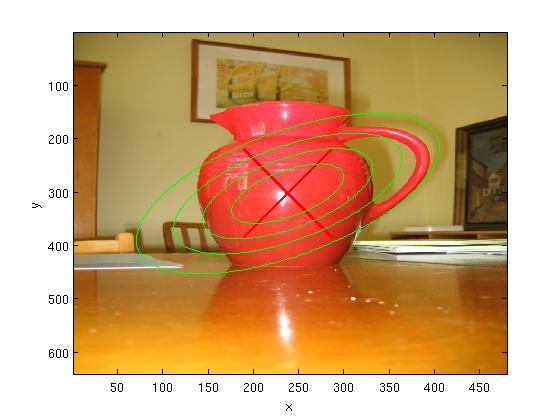
\includegraphics[width=0.6\textwidth]{images/kande1.png}
  \caption{The average of the probability of the pixels. The red cross marks the average, and the green lines are isoprobability curves of the gaussian distribution.}
  \label{fig:q1_9}
\end{figure}

\subsection*{Question 1.10}

When running the same code with the other image, the results are less successful, seen in figure \ref{fig:q1_10}.
The maximum likelyhood color is, correctly, much darker, which causes some of the brownish colors of the background to be identified as vase-colored.
As pixels with high probability now exist across the entire image, the average and spread are no longer a good indication of the location of the vase.

We can thus conclude that the method, while successful on some images, can not generally identify objects, as the background can interfere.

\begin{figure}[!htpb]
  \centering
  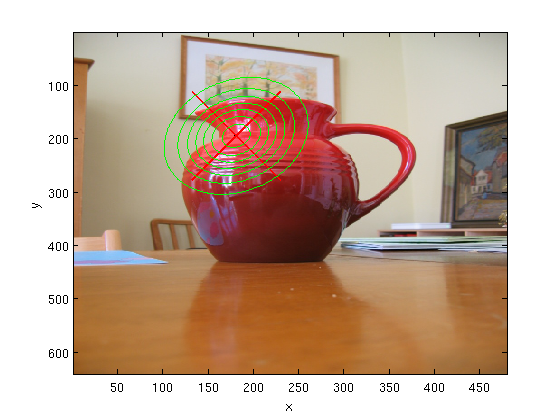
\includegraphics[width=0.6\textwidth]{images/kande2.png}
  \caption{The same data as in figure \ref{fig:q1_9}, but with the image "kande2.JPG".}
  \label{fig:q1_10}
\end{figure}

%%%%%%%%%%%%%%%%%%%%%%%%%%%%%%%%%%%%%%%%%%%%%%%%%%%%%%%%%%%%%%%%%%%%
% Formal stuff

%\bibliographystyle{abbrvnat}
%\bibliography{bibliography}
%\addcontentsline{toc}{chapter}{Litteratur

\end{document}

% vim: set tw=72 spell spelllang=en:
